\documentclass[tikz,border=6pt,multi=tikzpicture]{standalone}
\usepackage{amsmath}
\usepackage{pgfplots}
\pgfplotsset{compat=1.18}
\usetikzlibrary{arrows.meta,positioning,calc,fit}

\definecolor{epcgreen}{HTML}{1F684F}
\definecolor{epcgreen2}{HTML}{2F8F6B}
\definecolor{epcsoft}{HTML}{EAF6F0}
\definecolor{epcblue}{HTML}{3F7D8B}
\definecolor{epcgold}{HTML}{BD7A1E}
\definecolor{epcred}{HTML}{BF4D42}
\definecolor{epcink}{HTML}{172026}
\definecolor{epcgrid}{HTML}{DCE7E1}

\pgfplotsset{
  marketaxis/.style={
    width=10.4cm,
    height=6.8cm,
    axis lines=left,
    xmin=0,
    ymin=0,
    grid=both,
    major grid style={draw=epcgrid, line width=0.35pt},
    minor grid style={draw=epcgrid!55, line width=0.2pt},
    minor tick num=1,
    tick style={draw=none},
    ticklabel style={font=\scriptsize, color=epcink},
    label style={font=\small, color=epcink},
    legend style={draw=none, fill=white, font=\scriptsize, cells={anchor=west}},
    clip=false
  },
  marketline/.style={smooth, line width=1.25pt},
  marketguide/.style={dashed, draw=epcink!40, line width=0.55pt},
  marketpoint/.style={only marks, mark=*, mark size=2.4pt, draw=white, line width=0.5pt}
}

\tikzset{
  marketguide/.style={dashed, draw=epcink!40, line width=0.55pt}
}

\begin{document}

% 1. Fuentes del poder de mercado
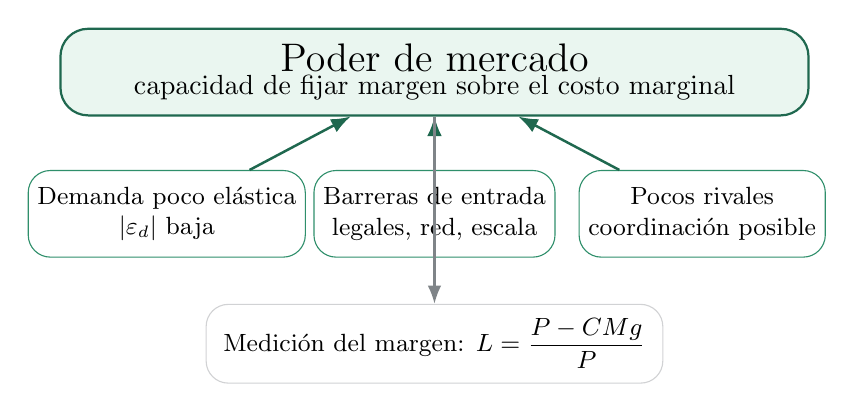
\begin{tikzpicture}[font=\small, >=Latex]
  \node[draw=epcgreen, fill=epcsoft, rounded corners=10pt, line width=0.8pt, minimum width=9.5cm, minimum height=1.1cm, align=center] (pm) at (0,1.8)
    {\Large Poder de mercado\\[-1mm]\normalsize capacidad de fijar margen sobre el costo marginal};
  \node[draw=epcgreen2, fill=white, rounded corners=8pt, minimum width=2.9cm, minimum height=1.1cm, align=center] (e) at (-3.4,0)
    {Demanda poco elástica\\$\lvert\varepsilon_d\rvert$ baja};
  \node[draw=epcgreen2, fill=white, rounded corners=8pt, minimum width=2.9cm, minimum height=1.1cm, align=center] (b) at (0,0)
    {Barreras de entrada\\legales, red, escala};
  \node[draw=epcgreen2, fill=white, rounded corners=8pt, minimum width=2.9cm, minimum height=1.1cm, align=center] (e2) at (3.4,0)
    {Pocos rivales\\coordinación posible};
  \node[draw=epcink!20, fill=white, rounded corners=8pt, minimum width=5.8cm, minimum height=1cm, align=center] (lerner) at (0,-1.65)
    {Medición del margen: $\displaystyle L=\frac{P-CMg}{P}$};
  \draw[->, epcgreen, line width=0.9pt] (e) -- (pm);
  \draw[->, epcgreen, line width=0.9pt] (b) -- (pm);
  \draw[->, epcgreen, line width=0.9pt] (e2) -- (pm);
  \draw[->, epcink!55, line width=0.8pt] (pm) -- (lerner);
\end{tikzpicture}

% 2. Monopolio
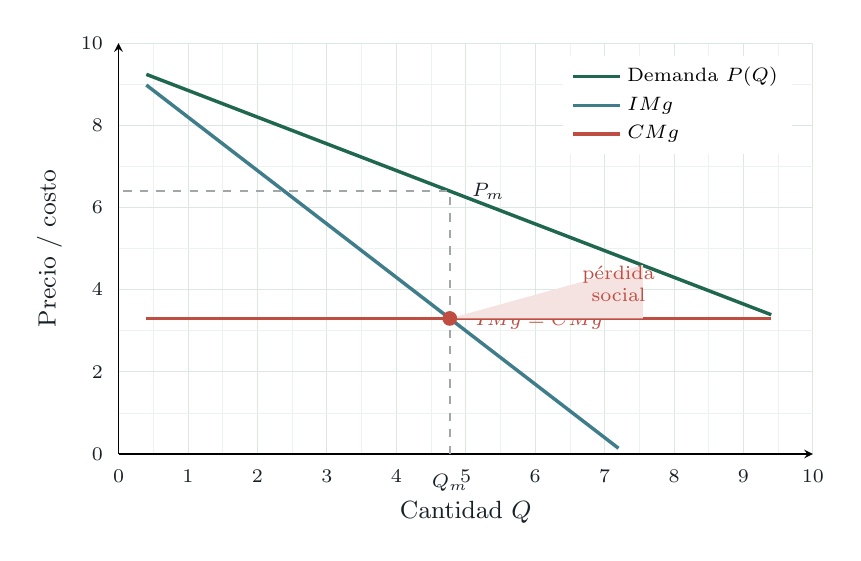
\begin{tikzpicture}
  \begin{axis}[marketaxis, xmax=10, ymax=10, xlabel={Cantidad $Q$}, ylabel={Precio / costo}, legend pos=north east]
    \addplot[marketline, color=epcgreen, domain=0.4:9.4, samples=2] {9.5-0.65*x};
    \addlegendentry{Demanda $P(Q)$}
    \addplot[marketline, color=epcblue, domain=0.4:7.2, samples=2] {9.5-1.3*x};
    \addlegendentry{$IMg$}
    \addplot[marketline, color=epcred, domain=0.4:9.4, samples=2] {3.3};
    \addlegendentry{$CMg$}
    \addplot[marketpoint, color=epcred] coordinates {(4.77,3.3)};
    \draw[marketguide] (axis cs:4.77,0) -- (axis cs:4.77,6.4) -- (axis cs:0,6.4);
    \node[font=\scriptsize, color=epcink, anchor=west] at (axis cs:4.95,6.4) {$P_m$};
    \node[font=\scriptsize, color=epcink, anchor=north] at (axis cs:4.77,-0.25) {$Q_m$};
    \node[font=\scriptsize, color=epcred, anchor=west] at (axis cs:5.0,3.25) {$IMg=CMg$};
    \fill[epcred!16] (axis cs:4.77,3.3) -- (axis cs:7.55,3.3) -- (axis cs:7.55,4.6) -- cycle;
    \node[font=\scriptsize, color=epcred, align=center] at (axis cs:7.2,4.15) {pérdida\\social};
  \end{axis}
\end{tikzpicture}

% 3. Monopolio natural
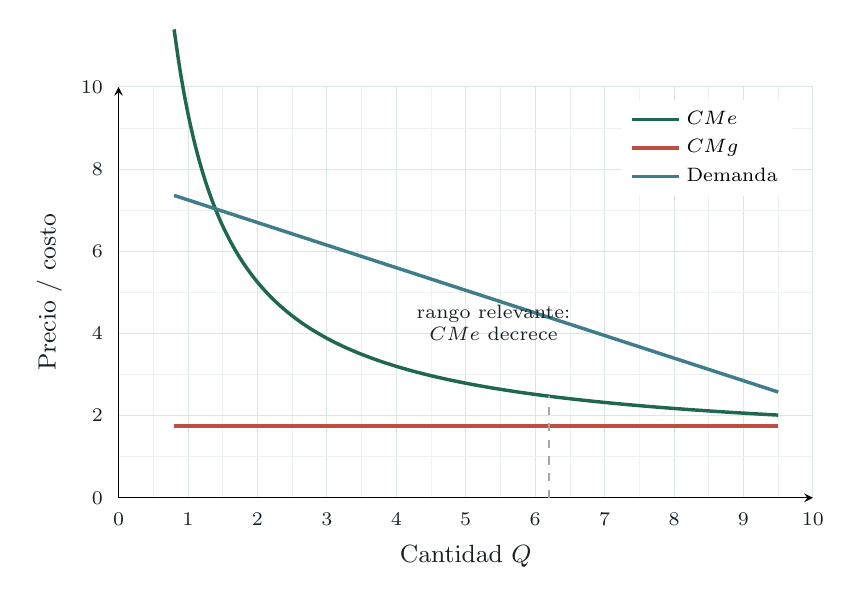
\begin{tikzpicture}
  \begin{axis}[marketaxis, xmax=10, ymax=10, xlabel={Cantidad $Q$}, ylabel={Precio / costo}, legend pos=north east]
    \addplot[marketline, color=epcgreen, domain=0.8:9.5, samples=120] {8.2/x + 1.15};
    \addlegendentry{$CMe$}
    \addplot[marketline, color=epcred, domain=0.8:9.5, samples=2] {1.75};
    \addlegendentry{$CMg$}
    \addplot[marketline, color=epcblue, domain=0.8:9.5, samples=2] {7.8-0.55*x};
    \addlegendentry{Demanda}
    \node[font=\scriptsize, color=epcink, align=center] at (axis cs:5.4,4.25) {rango relevante:\\$CMe$ decrece};
    \draw[marketguide] (axis cs:6.2,0) -- (axis cs:6.2,2.47);
  \end{axis}
\end{tikzpicture}

% 4. Discriminacion de precios
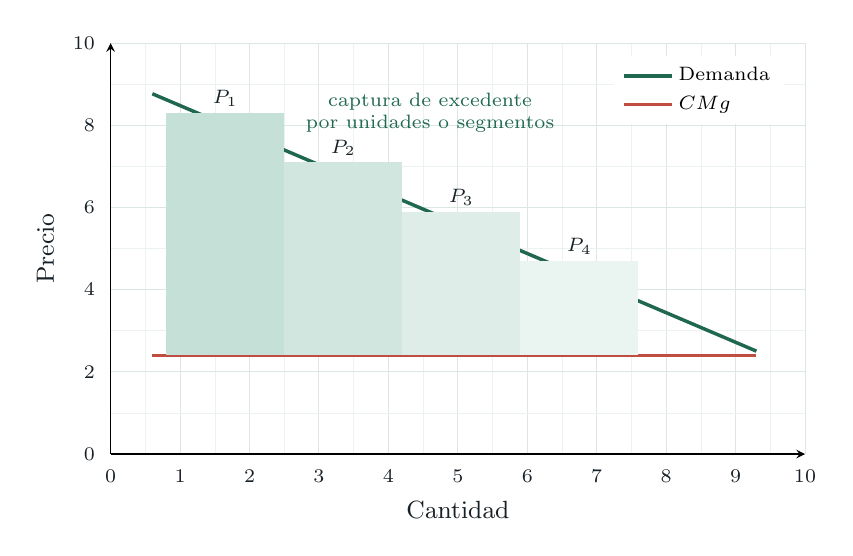
\begin{tikzpicture}
  \begin{axis}[marketaxis, xmax=10, ymax=10, xlabel={Cantidad}, ylabel={Precio}, legend pos=north east]
    \addplot[marketline, color=epcgreen, domain=0.6:9.3, samples=2] {9.2-0.72*x};
    \addlegendentry{Demanda}
    \addplot[marketline, color=epcred, domain=0.6:9.3, samples=2] {2.4};
    \addlegendentry{$CMg$}
    \fill[epcgreen2!28] (axis cs:0.8,2.4) rectangle (axis cs:2.5,8.3);
    \fill[epcgreen2!22] (axis cs:2.5,2.4) rectangle (axis cs:4.2,7.1);
    \fill[epcgreen2!16] (axis cs:4.2,2.4) rectangle (axis cs:5.9,5.9);
    \fill[epcgreen2!10] (axis cs:5.9,2.4) rectangle (axis cs:7.6,4.7);
    \node[font=\scriptsize, color=epcink] at (axis cs:1.65,8.65) {$P_1$};
    \node[font=\scriptsize, color=epcink] at (axis cs:3.35,7.45) {$P_2$};
    \node[font=\scriptsize, color=epcink] at (axis cs:5.05,6.25) {$P_3$};
    \node[font=\scriptsize, color=epcink] at (axis cs:6.75,5.05) {$P_4$};
    \node[font=\scriptsize, color=epcgreen, align=center] at (axis cs:4.6,8.3) {captura de excedente\\por unidades o segmentos};
  \end{axis}
\end{tikzpicture}

% 5. Monopsonio
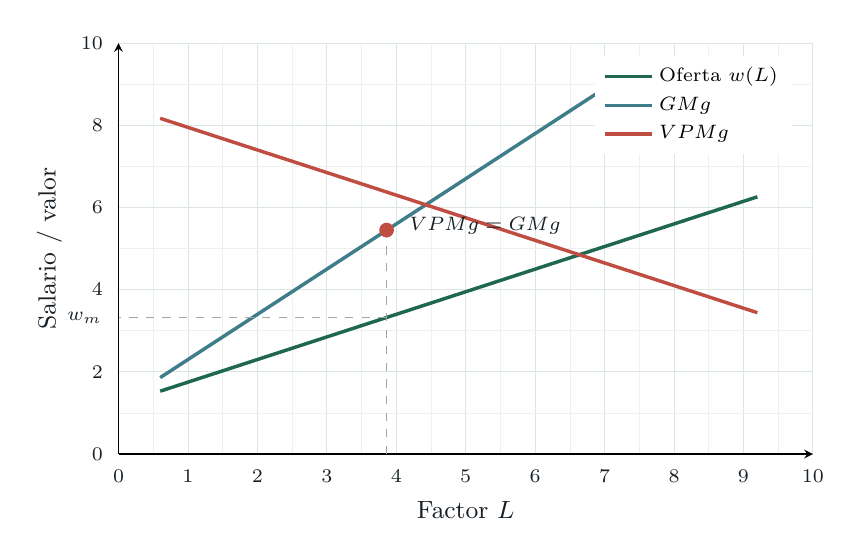
\begin{tikzpicture}
  \begin{axis}[marketaxis, xmax=10, ymax=10, xlabel={Factor $L$}, ylabel={Salario / valor}, legend pos=north east]
    \addplot[marketline, color=epcgreen, domain=0.6:9.2, samples=2] {1.2+0.55*x};
    \addlegendentry{Oferta $w(L)$}
    \addplot[marketline, color=epcblue, domain=0.6:7.6, samples=2] {1.2+1.1*x};
    \addlegendentry{$GMg$}
    \addplot[marketline, color=epcred, domain=0.6:9.2, samples=2] {8.5-0.55*x};
    \addlegendentry{$VPMg$}
    \addplot[marketpoint, color=epcred] coordinates {(3.86,5.45)};
    \draw[marketguide] (axis cs:3.86,0) -- (axis cs:3.86,5.45);
    \draw[marketguide] (axis cs:3.86,3.32) -- (axis cs:0,3.32);
    \node[font=\scriptsize, color=epcink, anchor=west] at (axis cs:4.05,5.55) {$VPMg=GMg$};
    \node[font=\scriptsize, color=epcink, anchor=east] at (axis cs:-0.1,3.32) {$w_m$};
  \end{axis}
\end{tikzpicture}

% 6. CR4 y HHI
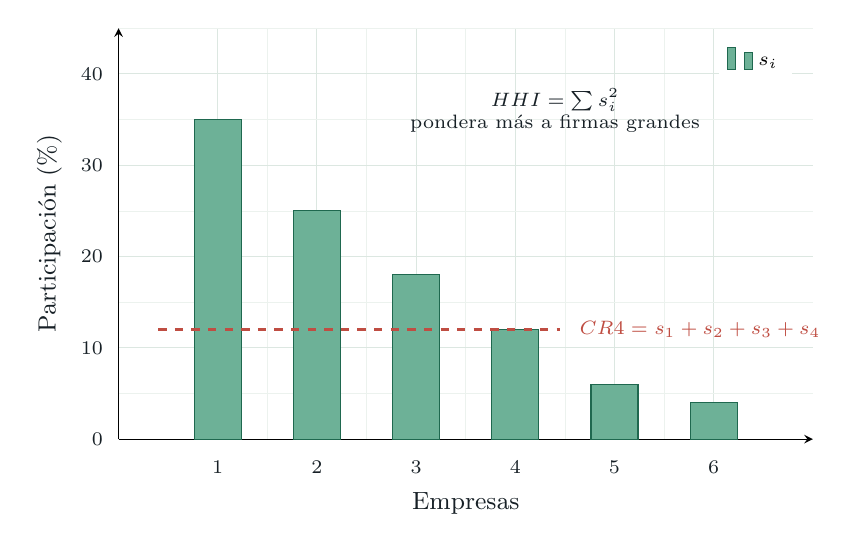
\begin{tikzpicture}
  \begin{axis}[marketaxis, ybar, bar width=17pt, xmax=7, ymax=45, xmin=0, xlabel={Empresas}, ylabel={Participación (\%)}, xtick={1,2,3,4,5,6}, legend pos=north east]
    \addplot[fill=epcgreen2!70, draw=epcgreen] coordinates {(1,35) (2,25) (3,18) (4,12) (5,6) (6,4)};
    \addlegendentry{$s_i$}
    \draw[epcred, line width=1pt, dashed] (axis cs:0.4,12) -- (axis cs:4.45,12);
    \node[font=\scriptsize, color=epcred, anchor=west] at (axis cs:4.55,12) {$CR4=s_1+s_2+s_3+s_4$};
    \node[font=\scriptsize, color=epcink, align=center] at (axis cs:4.4,36) {$HHI=\sum s_i^2$\\pondera más a firmas grandes};
  \end{axis}
\end{tikzpicture}

% 7. Oligopolio: mejores respuestas
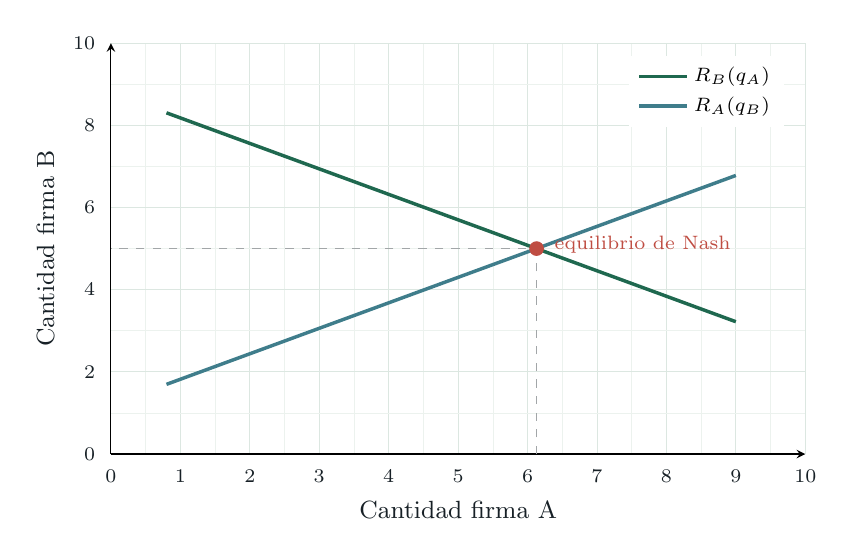
\begin{tikzpicture}
  \begin{axis}[marketaxis, xmax=10, ymax=10, xlabel={Cantidad firma A}, ylabel={Cantidad firma B}, legend pos=north east]
    \addplot[marketline, color=epcgreen, domain=0.8:9, samples=2] {8.8-0.62*x};
    \addlegendentry{$R_B(q_A)$}
    \addplot[marketline, color=epcblue, domain=0.8:9, samples=2] {1.2+0.62*x};
    \addlegendentry{$R_A(q_B)$}
    \addplot[marketpoint, color=epcred] coordinates {(6.13,5.0)};
    \node[font=\scriptsize, color=epcred, anchor=west] at (axis cs:6.25,5.1) {equilibrio de Nash};
    \draw[marketguide] (axis cs:6.13,0) -- (axis cs:6.13,5) -- (axis cs:0,5);
  \end{axis}
\end{tikzpicture}

% 8. Teoria de juegos: matriz legible
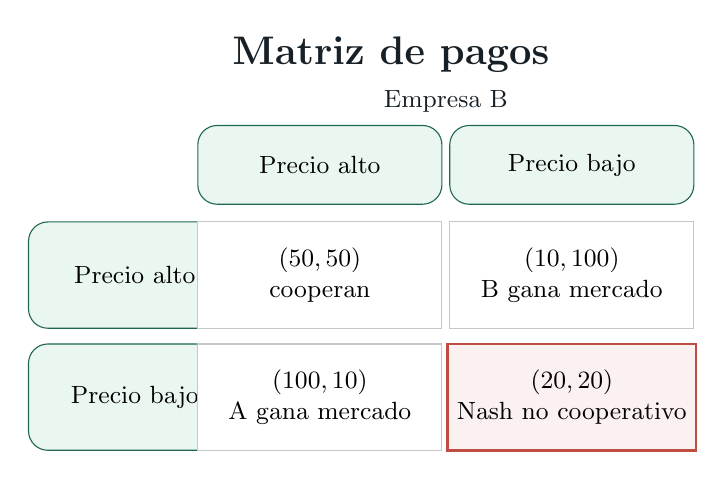
\begin{tikzpicture}[font=\small]
  \node[font=\Large\bfseries, color=epcink] at (0,3.15) {Matriz de pagos};
  \node[font=\small, color=epcink] at (-3.7,0.45) {Empresa A};
  \node[font=\small, color=epcink] at (0.7,2.55) {Empresa B};
  \node[draw=epcgreen, fill=epcsoft, rounded corners=7pt, minimum width=3.1cm, minimum height=1cm] at (-0.9,1.75) {Precio alto};
  \node[draw=epcgreen, fill=epcsoft, rounded corners=7pt, minimum width=3.1cm, minimum height=1cm] at (2.3,1.75) {Precio bajo};
  \node[draw=epcgreen, fill=epcsoft, rounded corners=7pt, minimum width=2.7cm, minimum height=1.35cm] at (-3.25,0.35) {Precio alto};
  \node[draw=epcgreen, fill=epcsoft, rounded corners=7pt, minimum width=2.7cm, minimum height=1.35cm] at (-3.25,-1.2) {Precio bajo};
  \node[draw=epcink!25, fill=white, minimum width=3.1cm, minimum height=1.35cm, align=center] at (-0.9,0.35) {$(50,50)$\\cooperan};
  \node[draw=epcink!25, fill=white, minimum width=3.1cm, minimum height=1.35cm, align=center] at (2.3,0.35) {$(10,100)$\\B gana mercado};
  \node[draw=epcink!25, fill=white, minimum width=3.1cm, minimum height=1.35cm, align=center] at (-0.9,-1.2) {$(100,10)$\\A gana mercado};
  \node[draw=epcred, fill=epcred!8, line width=1pt, minimum width=3.1cm, minimum height=1.35cm, align=center] at (2.3,-1.2) {$(20,20)$\\Nash no cooperativo};
\end{tikzpicture}

% 9. Estrategia dominante
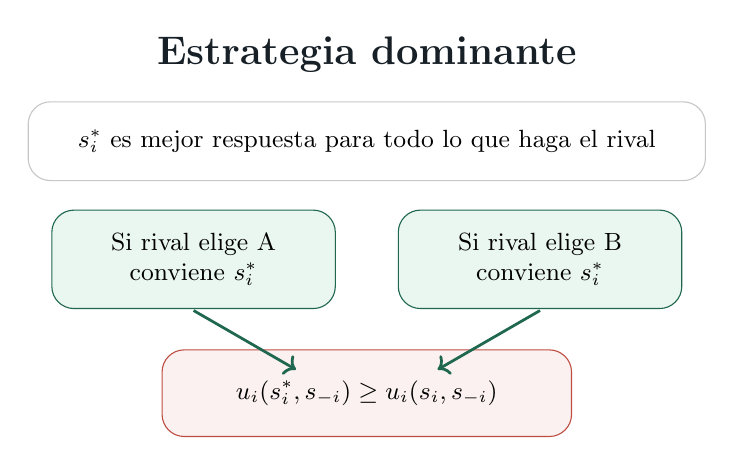
\begin{tikzpicture}[font=\small]
  \node[font=\Large\bfseries, color=epcink] at (0,3.05) {Estrategia dominante};
  \node[draw=epcink!25, fill=white, rounded corners=8pt, minimum width=8.6cm, minimum height=1.0cm, align=center] at (0,1.95)
    {$s_i^*$ es mejor respuesta para todo lo que haga el rival};
  \node[draw=epcgreen, fill=epcsoft, rounded corners=8pt, minimum width=3.6cm, minimum height=1.25cm, align=center] at (-2.2,0.45)
    {Si rival elige A\\conviene $s_i^*$};
  \node[draw=epcgreen, fill=epcsoft, rounded corners=8pt, minimum width=3.6cm, minimum height=1.25cm, align=center] at (2.2,0.45)
    {Si rival elige B\\conviene $s_i^*$};
  \node[draw=epcred, fill=epcred!8, rounded corners=8pt, minimum width=5.2cm, minimum height=1.1cm, align=center] at (0,-1.25)
    {$u_i(s_i^*,s_{-i})\ge u_i(s_i,s_{-i})$};
  \draw[->, epcgreen, line width=1pt] (-2.2,-0.2) -- (-0.9,-0.95);
  \draw[->, epcgreen, line width=1pt] (2.2,-0.2) -- (0.9,-0.95);
\end{tikzpicture}

% 10. Juegos repetidos
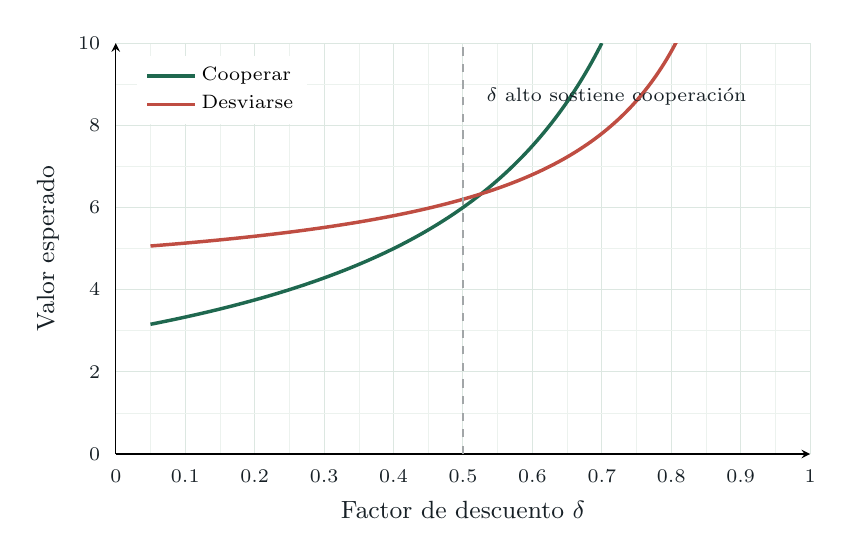
\begin{tikzpicture}
  \begin{axis}[marketaxis, clip=true, xmax=1, ymax=10, xlabel={Factor de descuento $\delta$}, ylabel={Valor esperado}, legend pos=north west]
    \addplot[marketline, color=epcgreen, domain=0.05:0.7, samples=80] {3/(1-x)};
    \addlegendentry{Cooperar}
    \addplot[marketline, color=epcred, domain=0.05:0.82, samples=80] {5+1.2*x/(1-x)};
    \addlegendentry{Desviarse}
    \draw[marketguide] (axis cs:0.5,0) -- (axis cs:0.5,10);
    \node[font=\scriptsize, color=epcink, anchor=west] at (axis cs:0.52,8.7) {$\delta$ alto sostiene cooperación};
  \end{axis}
\end{tikzpicture}

% 11. Informacion asimetrica
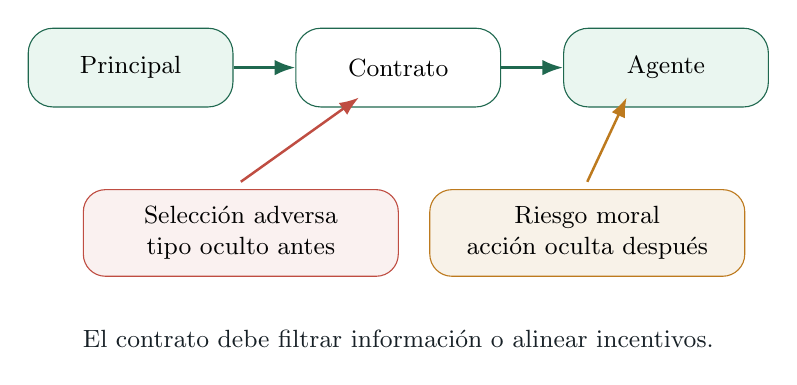
\begin{tikzpicture}[font=\small, >=Latex]
  \node[draw=epcgreen, fill=epcsoft, rounded corners=9pt, minimum width=2.6cm, minimum height=1cm] (p) at (-3.4,1.1) {Principal};
  \node[draw=epcgreen, fill=white, rounded corners=9pt, minimum width=2.6cm, minimum height=1cm] (c) at (0,1.1) {Contrato};
  \node[draw=epcgreen, fill=epcsoft, rounded corners=9pt, minimum width=2.6cm, minimum height=1cm] (a) at (3.4,1.1) {Agente};
  \draw[->, epcgreen, line width=1pt] (p) -- (c);
  \draw[->, epcgreen, line width=1pt] (c) -- (a);
  \node[draw=epcred, fill=epcred!8, rounded corners=8pt, align=center, minimum width=4cm, minimum height=1.1cm] at (-2.0,-1.0)
    {Selección adversa\\tipo oculto antes};
  \node[draw=epcgold, fill=epcgold!10, rounded corners=8pt, align=center, minimum width=4cm, minimum height=1.1cm] at (2.4,-1.0)
    {Riesgo moral\\acción oculta después};
  \draw[->, epcred, line width=0.9pt] (-2.0,-0.35) -- (-0.5,0.72);
  \draw[->, epcgold, line width=0.9pt] (2.4,-0.35) -- (2.9,0.72);
  \node[font=\small, color=epcink, align=center] at (0,-2.35) {El contrato debe filtrar información o alinear incentivos.};
\end{tikzpicture}

\end{document}
